%==================================================================
\frame{\frametitle{Different types of networks}

  \paragraph{Network =} natural and convenient way to represent ecological 'interactions' \refer{Bas09}

  \bigskip \bigskip \pause
  \paragraph{Many types of networks:} trophic, plant-pollinator, 'interaction'

  \bigskip \bigskip \pause
  \paragraph{Aim:} understand their organisations, i.e. analyse their {\sl topology}
  \begin{overprint}
    \onslide<4>
    \begin{tabular}{p{.35\textwidth}p{.55\textwidth}}
      \begin{tabular}{p{.35\textwidth}}
        Do trophic levels actually exist? \\
        \\
        {\tiny \url{en.wikipedia.org/wiki/Trophic_coherence}}
      \end{tabular}
      &
      \begin{tabular}{p{.55\textwidth}}
        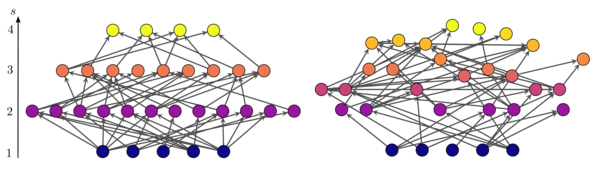
\includegraphics[trim=20 0 300 0, width=.35\textwidth, clip]{\figeco/WikipediaTrophicNetwork} \\
        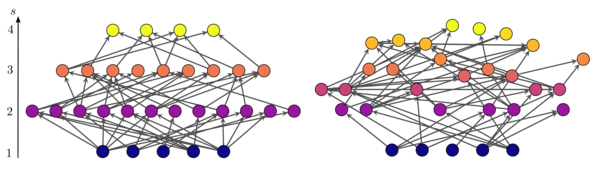
\includegraphics[trim=310 0 0 0, width=.35\textwidth, clip]{\figeco/WikipediaTrophicNetwork} 
      \end{tabular} 
    \end{tabular}
    \onslide<5>
    \begin{tabular}{p{.35\textwidth}p{.55\textwidth}}
      \begin{tabular}{p{.35\textwidth}}
        Generalist vs specialist pollinators?  \\
        \\
        {\tiny \url{seibutsu.biology.kyushu-u.ac.jp/~satake}}
      \end{tabular}
      &
      \begin{tabular}{p{.55\textwidth}}
        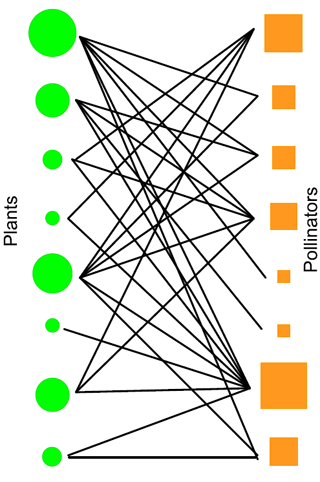
\includegraphics[height=.45\textwidth,angle=270]{\figeco/SatakePlantPollinatorNetwork}
      \end{tabular} 
    \end{tabular}
    \onslide<6>
    \begin{tabular}{p{.35\textwidth}p{.55\textwidth}}
      \begin{tabular}{p{.35\textwidth}}
        Is the network 'organized'? \\
        \\
        If so, how? \\
        \\
        {\tiny \url{www.allisonbarner.com}}
      \end{tabular}
      &
      \begin{tabular}{p{.55\textwidth}}
        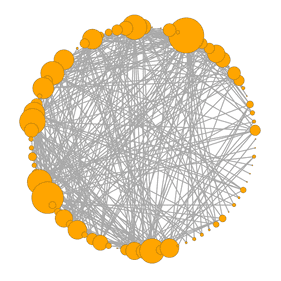
\includegraphics[width=.4\textwidth]{\figeco/BarnerEcologicalNetwork}
      \end{tabular} 
    \end{tabular}
  \end{overprint}
}
  
%==================================================================
\frame{\frametitle{Modelling approach}

  \paragraph{Mathematical counterpart:} 
  $$
  \text{ecological {\sl network}}
  \quad \leftrightarrow \quad
  \text{random {\sl graph}}  
  $$

  \bigskip \pause
  \paragraph{Random graph:}   $n$ nodes  = species, individuals, ... ($1 \leq i, j \leq n$), 
  $$
  Y_{ij} = \text{ 'value' of the edge between node $i$ and $j$}
  $$
  Random graph model = joint distribution of all edge values:
  $$
  p(\{Y_{ij}\}_{i, j})
  \qquad \rightarrow \qquad \simeq n^2 \text{ random variables}
  $$

  \bigskip \bigskip \pause
  \begin{tabular}{p{.35\textwidth}p{.6\textwidth}}
    \paragraph{Type of network:} & \paragraph{Type of edge:} \\ %~ \\
      directed / undirected & $Y_{ij} = Y_{ji}$ or not \\ %~ \\
      binary / valued ('weighted') & $Y_{ij} \in \{0, 1\}$ or $\Rbb$ \\ %~ \\
      multivariate ('multiplex') & $Y_{ij} \in \{0, 1\}^d$ or $\Rbb^d$ \\
      & or $\{0, 1\} \times \{a, b, c, d\} \times \Nbb \times \Rbb$
  \end{tabular}

}

%==================================================================
\frame{\frametitle{A model: what for?}

  Many different aims: \\~
  \begin{enumerate}[($a$)]
    \item \emphase{Mechanistic} model: pretends to encode the process that actually generated the data \\~
    \item \emphase{Empirical} model: enables to simulate data similar to the observed ones \\~ 
    \item \emphase{Null} model: serves as a reference to detect 'unexpected behaviors' 
  \end{enumerate}

  \bigskip \bigskip \pause
  \paragraph{Here,} focus on 
  \begin{itemize}
    \item ($b$) and ($c$): empirical and null models
    \item for binary networks (with some extensions)
  \end{itemize}


}
